%%%%%%%%%%%%%%%%%%%%%%%%%%%%%%%%%%%%%%%%%
%
% (c) 2020 by Jennifer Laaser
%
% This work is licensed under the Creative Commons Attribution-NonCommercial-ShareAlike 4.0 International License. To view a copy of this license, visit http://creativecommons.org/licenses/by-nc-sa/4.0/ or send a letter to Creative Commons, PO Box 1866, Mountain View, CA 94042, USA.
%
% The current source for these materials is accessible on Github: https://github.com/jlaaser/pogil-polymers
%
%%%%%%%%%%%%%%%%%%%%%%%%%%%%%%%%%%%%%%%%%

\renewcommand{\figpath}{content/intro/molecules-to-polymers/figs}
\renewcommand{\labelbase}{molecules-to-polymers}

\begin{activity}[From Molecules to Polymers]

\begin{instructornotes}

	This activity introduces students to the definition of the term \emph{polymer}, and key differences between small molecules and polymers.
	
	After completing this activity, students will be able to:
			\begin{enumerate}
				\item Define the term ``polymer''
				\item 
			\end{enumerate}
			
	\subsection*{Activity summary:}
	\begin{itemize}
		\item \textbf{Activity type:} Learning Cycle
		\item \textbf{Content goals:} Introduction to polymers
		\item \textbf{Process goals:} %https://pogil.org/uploads/attachments/cj54b5yts006cklx4hh758htf-process-skills-official-pogil-list-2015-original.pdf
			written communication, critical thinking, information processing
		\item \textbf{Duration:} TBD
		\item \textbf{Instructor preparation required:} none beyond knowledge of relevant content
		\item \textbf{Related textbook chapters:}
			\begin{itemize}
				\item \emph{Polymer Chemistry} (Hiemenz \& Lodge): section 1.2
			\end{itemize}
		%\item \textbf{Facilitation notes:}
		%	\begin{itemize}
		%		\item \dots
		%	\end{itemize}
	\end{itemize}

\end{instructornotes}

\begin{model}[Structures of Linear Hydrocarbons]

	Structures of several common linear hydrocarbons are shown below:
	
	\begin{center}
		\renewcommand{\arraystretch}{1.5}
		\begin{tabular}{ccc}
			\hline
			\textbf{Name} & \textbf{Formula} & \textbf{Structure}  \\\hline
			Ethane & \ce{C2H6} & 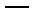
\includegraphics[scale=1]{\figpath/Model1_C2.pdf}\\%& 30 g/mol\\
			Butane & \ce{C4H10} & 
\includegraphics[scale=1]{\figpath/Model1_C4.pdf}\\%& 58 g/mol\\
			Hexane & \ce{C6H14} & 
\includegraphics[scale=1]{\figpath/Model1_C6.pdf}\\%& 86 g/mol\\
			Octane & \ce{C8H18} & 
\includegraphics[scale=1]{\figpath/Model1_C8.pdf}\\%& 114 g/mol\\
			Decane & \ce{C10H22} & 
\includegraphics[scale=1]{\figpath/Model1_C10.pdf}\\%& 142 g/mol
		\end{tabular}
	\end{center}


\end{model}


\begin{ctqs}

	\question Between each line of the table and the next...
		\begin{enumerate}
			\item ... how many carbon atoms are added to the molecule?
			
				\begin{solution}[0.25in]
				\end{solution}
				
			\item ... how many hydrogen atoms are added to the molecule?
			
				\begin{solution}[0.25in]
				\end{solution}
				
		\end{enumerate}
		
	\question Explain, in 1-2 complete sentences, why we might say that this series of molecules consists of ``repeating'' \ce{C2H4} units.
			
				\begin{solution}[2in]
				\end{solution}
				
		
	\question Predict the chemical formula of the next logical entry in the table, and draw its structure.
			
				\begin{solution}[1in]
				\end{solution}
		
	\question Consider a linear alkane with 100 carbon atoms. \label{\labelbase:ctq:100Calkane}
		\begin{enumerate}
			%\item What would the molecular weight of this molecule be?
			
			\item What would the chemical formula of this molecule be?
			
				\begin{solution}[1in]
				\end{solution}
			
			\item Do you \emph{want} to try to draw the full structure of this molecule?  Why or why not?
			
				\begin{solution}[1.5in]
				\end{solution}
		\end{enumerate}
\end{ctqs}

\begin{infobox}
	For convenience, large molecules with repeating structures are often abbreviated using the following notation:
	
	\centerline{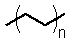
\includegraphics[scale=2]{\figpath/Model1_nrepeats.pdf}}
	
	Here, the repeat unit is enclosed in parentheses.  The repeat units are attached end-to-end, and the subscript $n$ indicates how many times this unit is repeated.  The portions outside of the parentheses are not part of the repeat unit, and indicate the chemical structure of the end-groups that ``cap'' the end of the molecule.
\end{infobox}

\begin{ctqs}
	\question Draw the full structure of the molecule shown in the following abbreviated structure: \label{\labelbase:ctq:abbrevbutane}
	
		\vspace{6pt}
		\centerline{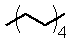
\includegraphics[scale=2]{\figpath/Model1_C10_abbreviated.pdf}}
		
		\begin{solution}[1.25in]
		\end{solution}
	
	\question Propose an analogous abbreviated structure for the 100-carbon linear alkane described in CTQ \ref{\labelbase:ctq:100Calkane}: \label{\labelbase:ctq:abbrev100}
		
		\begin{solution}[0.75in]
		\end{solution}
	
	\question What is the chemical formula \emph{of the repeat unit} for the structures in CTQs \ref{\labelbase:ctq:abbrevbutane} and \ref{\labelbase:ctq:abbrev100}?
		
		\begin{solution}[0.75in]
		\end{solution}
	
	\question What small molecule has the same chemical formula as this repeat unit?
		
		\begin{solution}[0.75in]
		\end{solution}
	
\end{ctqs}

\begin{infobox}
	When the number of repeat units is large, we often describe molecules with repeating structures as \emph{polymers}.  The word polymer comes from Greek: \emph{poly} means ``many'', while \emph{meros} means ``parts''.  Thus, a \emph{polymer} is a molecule composed of \emph{many} (often identical) \emph{parts}.
\end{infobox}

\begin{ctqs}
	\question Why might we describe molecules of the form
	
		\centerline{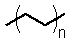
\includegraphics[scale=2]{\figpath/Model1_nrepeats.pdf}}
			
		as \emph{polyethylenes}?  Explain your answer in 1-2 complete sentences.
		
		\begin{solution}[2in]
		\end{solution}
\end{ctqs}

\clearpage
\begin{model}[Melting Points of Linear Hydrocarbons]
	\label{\labelbase:mdl:hydrocarbonmelting}

	The following plot shows the melting points of linear hydrocarbons with varying numbers of carbon atoms:
	
	\vspace{6pt}
	
	\centerline{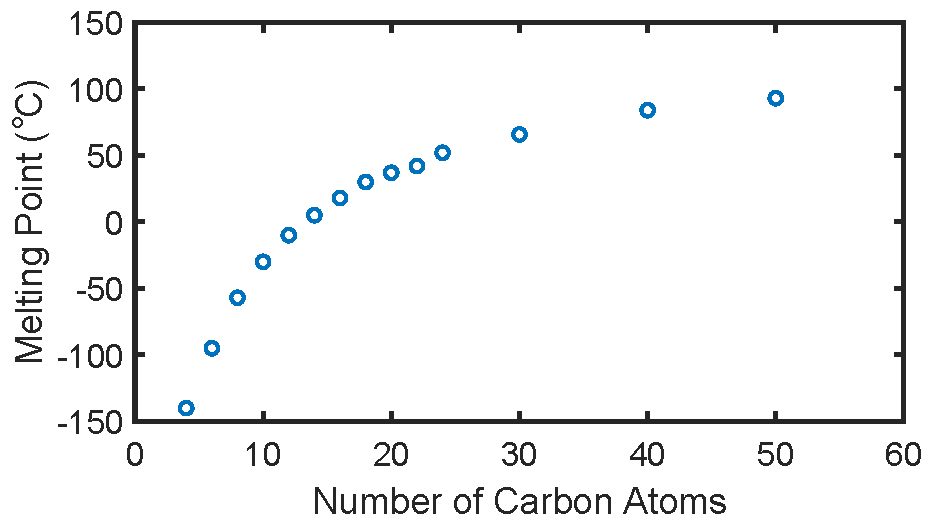
\includegraphics[width=0.7\textwidth]{\figpath/meltingpoints_cleaned.pdf}}
	
	\vspace{6pt}

\end{model}

\begin{ctqs}

	%\question In 2-3 complete sentences, describe the trend that you observe in this data.
	
		%\begin{solution}[2in]
		%\end{solution}
	
	\question Consider a sample of ethane molecules.  What type(s) of interactions (e.g. covalent, ionic, hydrogen bonding, van der Waals, etc.) do you expect to govern interactions between these molecules?%, and why?  %Briefly explain your team's reasoning.
	
		\begin{solution}[0.5in]
		\end{solution}
	
	\question As the number of carbon atoms in the molecule increases, do you expect the strength of these intermolecular interactions increase, decrease, or stay the same? \label{\labelbase:ctq:interactionstrength}
	
		\begin{solution}[0.5in]
		\end{solution}
	
	\question Using your answer to CTQ \ref{\labelbase:ctq:interactionstrength}, explain the origin of the trend observed in Model \ref{\labelbase:mdl:hydrocarbonmelting} in 1-2 complete sentences.
	
		\begin{solution}[2in]
		\end{solution}
	
	\question Based on the data presented in Model \ref{\labelbase:mdl:hydrocarbonmelting}, what do you expect to happen to the melting temperature as the number of carbon atoms gets very large (1000 or 10000 or more)?  Briefly explain your team's reasoning.
	
		\begin{solution}[2in]
		\end{solution}
	
	\question The melting temperature of polyethylene is typically quoted as approximately 120~${}^\circ$C.  In your group's judgment, how many carbon atoms are necessary before the melting behavior begins to ``look'' more like the polymer than like a small molecule?  Explain your choice in 2-3 complete sentences. \label{\labelbase:ctq:npolymer}
	
		\begin{solution}[2in]
		\end{solution}
	
	%\question How many repeat units does this number of carbons correspond to?
	
	%	\begin{solution}[0.5in]
	%	\end{solution}
			
\end{ctqs}

		

\begin{exercises}

	\exercise How many repeat units does the number of carbon atoms you identified in CTQ \ref{\labelbase:ctq:npolymer} correspond to?

	\exercise In this class, we will primarily use the word ``polymer'' to describe large molecules with repeating structures.  Another word commonly used in this field, however, is ``macromolecule''.  Why is this also a reasonable term for describing this class of molecules, and does it capture any important features that are missed by the word ``polymer''?
	
\end{exercises}


%\begin{problems}

%	\problem First exercise
%	\problem Second exercise
	
%\end{problems}


	
\end{activity}